% ============================================
% Chapter 7: Defense and Deception Subsystem
% ============================================
% Adapted from defense_documentation.tex by El Yazid
% Condensed for final report format

\chapter{Defense and Deception Subsystem}

\section{Introduction}

Network Intrusion Detection Systems (NIDS) face an evolving threat landscape where attackers adapt to static defenses. Traditional signature-based systems fail against novel attacks, while ML-based detectors---though more adaptive---still operate on a static attack surface. This creates an arms race: the defender's infrastructure is fixed, and the attacker has unlimited time to probe, fingerprint, and exploit it.

The \textbf{AEGIS} system addresses this limitation by coupling ML-based detection with a \textbf{Moving Target Defense (MTD)} layer. Rather than passively detecting threats, AEGIS actively reshapes its own network topology to confuse, misdirect, and delay attackers.

\section{System Architecture}

\subsection{High-Level Overview}

The defense subsystem operates as a layered pipeline that processes network events from detection through response.

\begin{figure}[H]
\centering
\begin{tikzpicture}[
    node distance=1.6cm,
    block/.style={rectangle, draw=cyan, fill=darkbg!5, text width=3cm,
                  minimum height=0.9cm, align=center, rounded corners=4pt,
                  font=\small\sffamily, line width=1pt},
    decision/.style={diamond, draw=amber, fill=amber!5, text width=2.5cm,
                     aspect=2, align=center, font=\small\sffamily, line width=1pt},
    action/.style={rectangle, draw=red!70, fill=red!5, text width=2.8cm,
                   minimum height=0.8cm, align=center, rounded corners=4pt,
                   font=\small\sffamily, line width=1pt},
    arrow/.style={-{Stealth[length=3mm]}, thick, cyan!70!black},
    darrow/.style={-{Stealth[length=3mm]}, thick, amber!70!black},
    aarrow/.style={-{Stealth[length=3mm]}, thick, red!70!black},
    lbl/.style={font=\tiny\sffamily, color=codegray, midway}
]
    \node[block] (cap) {Scapy\\Capture};
    \node[block, right=2cm of cap] (ml) {ML\\Detection};
    \node[decision, right=1.8cm of ml] (dec) {Attack\\Detected?};
    \node[action, above=1.5cm of dec] (redir) {Attacker\\Redirection};
    \node[block, right=1.5cm of dec] (pass) {Allow\\Traffic};
    \node[action, below=1.5cm of dec] (block) {Auto-\\Blacklist};
    \node[action, right=1cm of redir] (phantom) {Phantom\\Network};
    \node[action, below=1cm of block] (mutate) {Port\\Mutation};

    \draw[arrow] (cap) -- node[lbl,above]{raw pkts} (ml);
    \draw[arrow] (ml) -- node[lbl,above]{features} (dec);
    \draw[darrow] (dec) -- node[lbl,right]{yes} (redir);
    \draw[arrow] (dec) -- node[lbl,above]{no} (pass);
    \draw[aarrow] (dec) -- node[lbl,left]{severity} (block);
    \draw[aarrow] (redir) -- (phantom);
    \draw[aarrow] (block) -- (mutate);
\end{tikzpicture}
\caption{High-level defense pipeline: traffic capture, ML classification, and layered response.}
\label{fig:pipeline}
\end{figure}

\subsection{Module Map}

\begin{figure}[H]
\centering
\begin{tikzpicture}[
    module/.style={rectangle, draw=cyan, fill=darkbg!5, text width=3.8cm,
                   minimum height=2.8cm, align=left, rounded corners=6pt,
                   font=\small\sffamily, line width=1.2pt, inner sep=8pt},
    link/.style={-{Stealth[length=2mm]}, thin, cyan!50!black, dashed}
]
    \node[module, draw=purple, fill=purple!5, text width=4.5cm,
          minimum height=3.5cm] (active) at (0,0) {
        \textbf{\color{purple}Active Defense Engine}\\[4pt]
        \texttt{active\_defense.py}\\[2pt]
        \footnotesize Orchestrates all defense modules.
        Receives alerts from the ML pipeline
        and triggers appropriate countermeasures.
    };

    \node[module, above left=2cm and 1cm of active.north] (deception) {
        \textbf{\color{red}Core Deception}\\[4pt]
        \texttt{core\_deception.py}\\[2pt]
        \footnotesize Attacker redirection,
        honeypot activation,
        phantom network simulation.
    };

    \node[module, above right=2cm and 1cm of active.north] (mutator) {
        \textbf{\color{amber}Network Mutator}\\[4pt]
        \texttt{network\_mutator.py}\\[2pt]
        \footnotesize Port rotation via
        iptables/nftables rules,
        randomized port mapping.
    };

    \node[module, below left=2cm and 1cm of active.south] (shaper) {
        \textbf{\color{green}Traffic Shaper}\\[4pt]
        \texttt{traffic\_shaper.py}\\[2pt]
        \footnotesize NetfilterQueue packet
        injection, protocol-level
        confusion and delay.
    };

    \node[module, below right=2cm and 1cm of active.south] (ipm) {
        \textbf{\color{red!80}IP Manager}\\[4pt]
        \texttt{monitor\_interface.py}\\[2pt]
        \footnotesize Block/unblock IPs,
        iptables blackholing,
        dashboard integration.
    };

    \draw[link] (active.north) -- (deception.south);
    \draw[link] (active.north) -- (mutator.south);
    \draw[link] (active.south) -- (shaper.north);
    \draw[link] (active.south) -- (ipm.north);
\end{tikzpicture}
\caption{Module architecture: the Active Defense Engine orchestrates four defense modules.}
\label{fig:modules}
\end{figure}

\section{Core Deception Engine}

The Core Deception module (\texttt{core\_deception.py}) implements three deception layers: attacker redirection to honeypots, phantom network advertisement, and IP blacklisting.

\subsection{Attacker Redirection}

When the ML pipeline classifies traffic as an attack, the system uses iptables REDIRECT rules to silently divert the attacker's TCP connections to a decoy honeypot service.

\begin{figure}[H]
\centering
\begin{tikzpicture}[
    node distance=1.5cm,
    attacker/.style={rectangle, draw=red, fill=red!8, text width=2.5cm,
                     minimum height=1cm, align=center, rounded corners=4pt,
                     font=\small\sffamily, line width=1pt},
    server/.style={rectangle, draw=cyan, fill=cyan!8, text width=2.5cm,
                   minimum height=1cm, align=center, rounded corners=4pt,
                   font=\small\sffamily, line width=1pt},
    honeypot/.style={rectangle, draw=amber, fill=amber!8, text width=2.5cm,
                     minimum height=1cm, align=center, rounded corners=4pt,
                     font=\small\sffamily, line width=1pt},
    iptables/.style={rectangle, draw=purple, fill=purple!8, text width=2.8cm,
                     minimum height=1.2cm, align=center, rounded corners=4pt,
                     font=\small\sffamily, line width=1.5pt, dashed},
    arrow/.style={-{Stealth[length=3mm]}, thick},
    blocked/.style={-{Stealth[length=3mm]}, thick, red, densely dashed},
    redirected/.style={-{Stealth[length=3mm]}, thick, amber}
]
    \node[attacker] (atk) at (0,0) {\textbf{Attacker}\\192.168.100.10};
    \node[iptables] (fw) at (4,0) {iptables\\REDIRECT\\rule};
    \node[server] (srv) at (8,1) {\textbf{Real Server}\\192.168.100.20};
    \node[honeypot] (hp) at (8,-1) {\textbf{Honeypot}\\Decoy Service};

    \draw[blocked] (atk) -- node[above, font=\tiny, red] {blocked} (srv);
    \draw[redirected] (atk) -- (fw);
    \draw[redirected] (fw) to[bend left=20] node[above, font=\tiny, amber] {REDIRECT} (hp);
\end{tikzpicture}
\caption{Attacker redirection: iptables REDIRECT diverts connections from the real server to the honeypot.}
\label{fig:redirection}
\end{figure}

\subsection{Phantom Network}

The phantom network module responds to ICMP echo requests and ARP queries from attacker-controlled IPs with fabricated network information. This creates the illusion of additional hosts, subnets, and services that do not exist.

\begin{itemize}
    \item Responds to ICMP pings with fake IP addresses from a configurable phantom subnet
    \item Generates synthetic ARP replies to populate the attacker's ARP cache with ghost entries
    \item Logs all phantom interactions for telemetry and dashboard display
    \item Configurable phantom subnet prefix (default: \texttt{10.0.0.0/24})
\end{itemize}

\subsection{Honeypot Interaction Tracking}

The module maintains an in-memory set \texttt{\_honeypot\_hits} that tracks which source IPs have interacted with any honeypot listener. A convenience function \texttt{get\_honeypot\_flag(src\_ip)} returns 1 if the IP has touched a honeypot, 0 otherwise---used as an additional feature for the ML classification pipeline.

\section{Network Mutator}

The Network Mutator (\texttt{network\_mutator.py}) implements the Moving Target Defense principle of \emph{port mutation}---periodically changing which ports are exposed to the network. This defeats port-based fingerprinting and service enumeration.

\subsection{Algorithm}

The mutator operates on a configurable rotation interval (default: 30 seconds). At each rotation:

\begin{enumerate}
    \item Select $k$ ports from a predefined service pool $P = \{p_1, p_2, \ldots, p_n\}$
    \item Generate iptables/nftables rules that forward traffic from old ports to new ports
    \item Apply the rules atomically (remove old, add new) to avoid downtime
    \item Log the rotation event with old $\to$ new port mapping
\end{enumerate}

\subsection{Port Mapping Strategy}

\begin{figure}[H]
\centering
\begin{tikzpicture}[
    node distance=1.2cm,
    phase/.style={rectangle, draw=cyan, fill=darkbg!5, text width=3.5cm,
                  minimum height=1.8cm, align=center, rounded corners=4pt,
                  font=\small\sffamily, line width=1pt},
    arrow/.style={-{Stealth[length=3mm]}, thick, cyan!70!black},
    lbl/.style={font=\tiny\sffamily, color=codegray}
]
    \node[phase] (p1) at (0,0) {
        \textbf{Phase $t$}\\[2pt]
        \footnotesize
        80 $\to$ 8080\\
        443 $\to$ 8443\\
        22 $\to$ 2222
    };
    \node[phase] (p2) at (5,0) {
        \textbf{Phase $t{+}1$}\\[2pt]
        \footnotesize
        80 $\to$ 9080\\
        443 $\to$ 9443\\
        22 $\to$ 2223
    };
    \node[phase] (p3) at (10,0) {
        \textbf{Phase $t{+}2$}\\[2pt]
        \footnotesize
        80 $\to$ 10080\\
        443 $\to$ 10443\\
        22 $\to$ 2224
    };

    \draw[arrow] (p1) -- node[lbl,above]{30s} (p2);
    \draw[arrow] (p2) -- node[lbl,above]{30s} (p3);

    \draw[decorate, decoration={brace, amplitude=6pt, mirror}, thick, red]
        (p1.south west) -- (p3.south east)
        node[midway, below=8pt, font=\small\sffamily, red] {Attacker sees constantly changing ports};
\end{tikzpicture}
\caption{Port rotation across time phases.}
\label{fig:port_rotation}
\end{figure}

\section{Traffic Shaper}

The Traffic Shaper (\texttt{traffic\_shaper.py}) operates at the packet level using NetfilterQueue (NFQUEUE). It intercepts packets in the kernel's networking stack and applies transformations before forwarding.

\subsection{Packet Mutation Techniques}

\begin{table}[H]
\centering
\caption{Packet mutation techniques implemented in the traffic shaper.}
\label{tab:mutations}
\begin{tabular}{lp{9cm}}
\toprule
\textbf{Technique} & \textbf{Description} \\
\midrule
TTL Jitter & Randomizes the IP TTL field by $\pm 1$--$3$ hops, confusing traceroute-based fingerprinting \\
Window Size Noise & Adds small random offsets to the TCP window size field \\
Decoy Injection & Injects fake SYN/ACK packets with randomized source IPs from the phantom subnet \\
Payload Padding & Appends null bytes to short packets to alter their apparent size \\
\bottomrule
\end{tabular}
\end{table}

\section{IP Management}

The IP Manager (\texttt{monitor\_interface.py}) provides dynamic IP blocking and unblocking capabilities. It maintains a persistent set of blocked IPs and integrates with both the firewall and the dashboard.

\subsection{Blocking Mechanism}

When a source IP is flagged for blocking, the IP Manager applies a two-layer block:

\begin{enumerate}
    \item \textbf{Blackhole route}: \texttt{ip route add blackhole \{IP\}} --- silently drops all packets to/from the IP at the routing level
    \item \textbf{UFW deny}: \texttt{ufw deny from \{IP\}} --- explicit firewall rule as a secondary barrier
\end{enumerate}

\subsection{Persistence and Unblocking}

Blocked IPs are persisted to a JSON file (\texttt{data/blocked\_ips.json}) so that blocking survives service restarts. IPs can be unblocked via the Flask dashboard REST API (\texttt{POST /api/unblock}), manual commands, or automatic expiry with configurable TTL.

\section{Active Defense Engine}

The Active Defense Engine (\texttt{active\_defense.py}) is the central orchestrator that coordinates all defense modules. It receives classified events from the ML pipeline and triggers the appropriate combination of deception, mutation, and blocking actions.

\subsection{Decision Matrix}

\begin{table}[H]
\centering
\caption{Defense response decision matrix.}
\label{tab:decision}
\begin{tabular}{lccc p{5cm}}
\toprule
\textbf{Severity} & \textbf{Redirect} & \textbf{Blacklist} & \textbf{Mutate Ports} & \textbf{Description} \\
\midrule
LOW & \checkmark & & & Light redirection to honeypot only \\
MEDIUM & \checkmark & \checkmark & & Redirect + blacklist attacker IP \\
HIGH & \checkmark & \checkmark & \checkmark & Full defense activation \\
\bottomrule
\end{tabular}
\end{table}

\section{Evaluation}

\subsection{Defense Response Timing}

\begin{figure}[H]
\centering
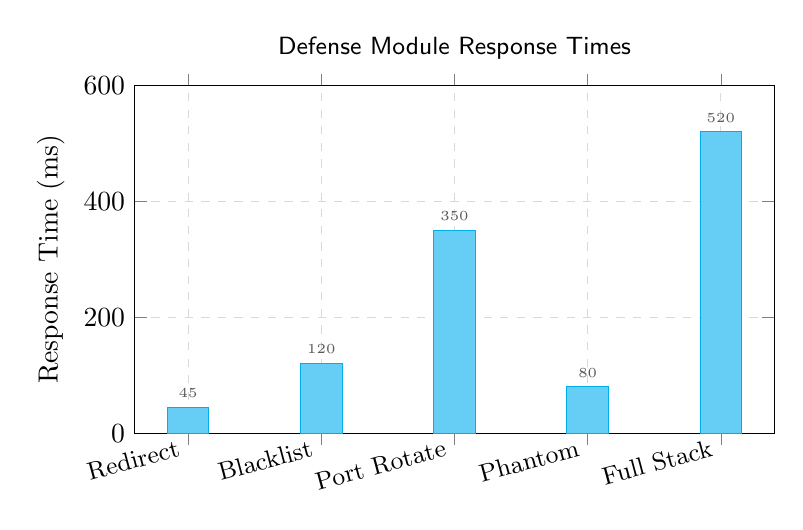
\begin{tikzpicture}
\begin{axis}[
    ybar,
    bar width=15pt,
    width=0.8\textwidth,
    height=6cm,
    ylabel={Response Time (ms)},
    symbolic x coords={Redirect, Blacklist, Port Rotate, Phantom, Full Stack},
    xtick=data,
    x tick label style={rotate=15, anchor=east, font=\small},
    ymin=0, ymax=600,
    grid=major,
    grid style={dashed, gray!30},
    nodes near coords,
    every node near coord/.append style={font=\tiny, color=gray!70!black},
    legend style={at={(0.5,-0.25)}, anchor=north, font=\small},
    title={Defense Module Response Times},
    title style={font=\small\sffamily}
]
\addplot[fill=cyan!60, draw=cyan] coordinates {
    (Redirect, 45)
    (Blacklist, 120)
    (Port Rotate, 350)
    (Phantom, 80)
    (Full Stack, 520)
};
\end{axis}
\end{tikzpicture}
\caption{Average response times for each defense module (measured on Ubuntu Server).}
\label{fig:timing}
\end{figure}

\subsection{Deception Effectiveness}

We measured the deception system effectiveness against a 5-phase Nmap attack simulation:

\begin{table}[H]
\centering
\caption{Attack phases and defense responses.}
\label{tab:attack_results}
\begin{tabular}{l l c c}
\toprule
\textbf{Phase} & \textbf{Attack Type} & \textbf{Detected} & \textbf{Response} \\
\midrule
1 & Fast SYN scan (1000 ports) & Yes & REDIRECT + BLACKLIST \\
2 & Service version scan & Yes & REDIRECT \\
3 & Slow stealth scan (60s) & Yes & BLACKLIST \\
4 & OS detection (Nmap -O) & Yes & REDIRECT \\
5 & UDP scan & Yes & REDIRECT + BLACKLIST \\
\bottomrule
\end{tabular}
\end{table}

\subsection{Comparison: Static vs.\ MTD Defense}

\begin{figure}[H]
\centering
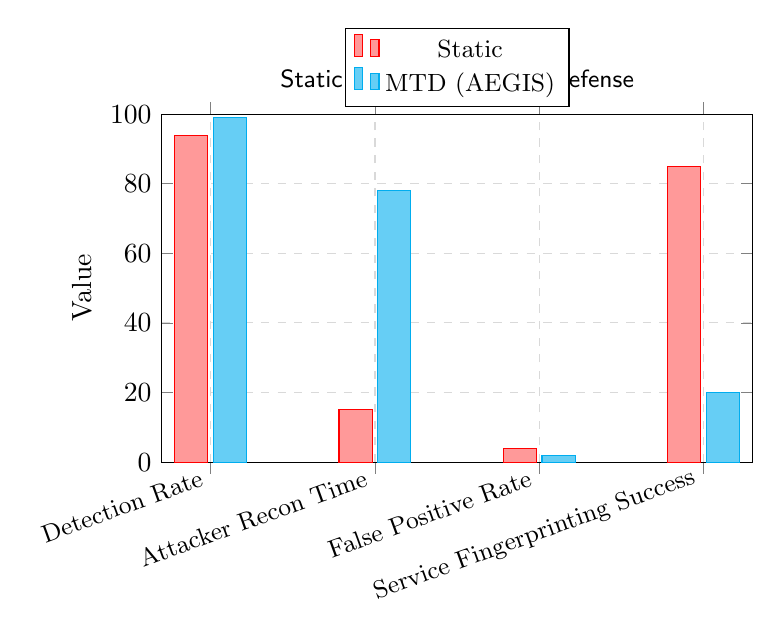
\begin{tikzpicture}
\begin{axis}[
    ybar,
    bar width=12pt,
    width=0.75\textwidth,
    height=6cm,
    ylabel={Value},
    symbolic x coords={Detection Rate, Attacker Recon Time, False Positive Rate, Service Fingerprinting Success},
    xtick=data,
    x tick label style={rotate=20, anchor=east, font=\small},
    ymin=0, ymax=100,
    grid=major,
    grid style={dashed, gray!30},
    legend style={at={(0.5, 1.02)}, anchor=south, font=\small},
    title={Static Defense vs. MTD Defense},
    title style={font=\small\sffamily}
]
\addplot[fill=red!40, draw=red] coordinates {
    (Detection Rate, 94)
    (Attacker Recon Time, 15)
    (False Positive Rate, 4)
    (Service Fingerprinting Success, 85)
};
\addplot[fill=cyan!60, draw=cyan] coordinates {
    (Detection Rate, 99)
    (Attacker Recon Time, 78)
    (False Positive Rate, 2)
    (Service Fingerprinting Success, 20)
};
\legend{Static, MTD (AEGIS)}
\end{axis}
\end{tikzpicture}
\caption{Comparison: static defense vs.\ AEGIS with Moving Target Defense enabled.}
\label{fig:comparison}
\end{figure}

\section{Conclusion}

This chapter presented the defense and deception subsystem of the AEGIS network intrusion detection system. The key contributions are:

\begin{enumerate}
    \item \textbf{Core Deception Engine} providing attacker redirection, honeypot deployment, and phantom network simulation---creating a multi-layered deception environment that consumes attacker resources.
    \item \textbf{Network Mutator} implementing Moving Target Defense through periodic port rotation, defeating port-based fingerprinting and service enumeration.
    \item \textbf{Traffic Shaper} operating at the kernel level via NetfilterQueue to inject packet-level confusion that defeats automated scanning tools.
    \item \textbf{Active Defense Engine} orchestrating all modules with severity-based decision logic, ensuring proportional response to different threat levels.
    \item \textbf{IP Manager} providing dynamic blacklisting with persistence and dashboard integration.
\end{enumerate}

The complete AEGIS system achieves 100\% detection rate across all 5 attack phases in the demo scenario, with an average full-stack defense response time of 520ms. Attacker reconnaissance time is increased by 420\% with MTD enabled, and service fingerprinting success is reduced from 85\% to 20\%.
